\documentclass[a5paper,portrait]{article}

% Encodage et langue
\usepackage[utf8]{inputenc}
\usepackage[T1]{fontenc}
\usepackage[french]{babel}

% Mise en page et graphiques
\usepackage{geometry}
\geometry{margin=1.5cm}
\usepackage{graphicx}
\usepackage{caption}
\usepackage{subcaption}
\usepackage{array}
\usepackage{tabularx}
\usepackage{longtable}
\usepackage{multicol}
\usepackage{enumitem}
\usepackage{fancyhdr}
\usepackage{titlesec}
\usepackage{xcolor}
\usepackage{lmodern} % Police moderne et sans-serif
\usepackage{tcolorbox}

% Palette de couleurs sobres
\definecolor{mainblue}{HTML}{2D4159}
\definecolor{lightgray}{HTML}{F5F6FA}
\definecolor{accent}{HTML}{F7B32B}

% Styles de titres modernes
\titleformat{\section}
  {\color{mainblue}\sffamily\LARGE\bfseries}
  {}{0pt}{}
\titleformat{\subsection}
  {\color{accent}\sffamily\large\bfseries}
  {}{0pt}{}

% En-tête et pied de page sobres
\pagestyle{fancy}
\fancyhf{}
\fancyhead[L]{\color{mainblue}\sffamily Notice d'Assemblage}
\fancyhead[R]{\color{mainblue}\sffamily\thepage}
\renewcommand{\headrulewidth}{0pt}

% Listes compactes et sans puce
\setlist[itemize]{left=0pt, label=--, topsep=2pt}
\setlist[enumerate]{topsep=2pt}

% Tableaux épurés
\renewcommand{\arraystretch}{1.2}
\setlength{\tabcolsep}{8pt}

% Fond de page clair (optionnel)
%\pagecolor{lightgray}

\begin{document}

\begin{titlepage}
    %\begin{minipage}[t][0.95\textheight][t]{0.48\textwidth}
    %\end{minipage}%
    \hfill
    %\begin{minipage}[t][0.95\textheight][t]{0.48\textwidth}
        \centering
        \vspace*{2cm}
        {\color{mainblue}\sffamily\Huge Notice d'Assemblage}\\[1cm]
        {\color{accent}\sffamily\Large Modèle inspiré par IKEA et LEGO}\\[1.5cm]
        \begin{center}
            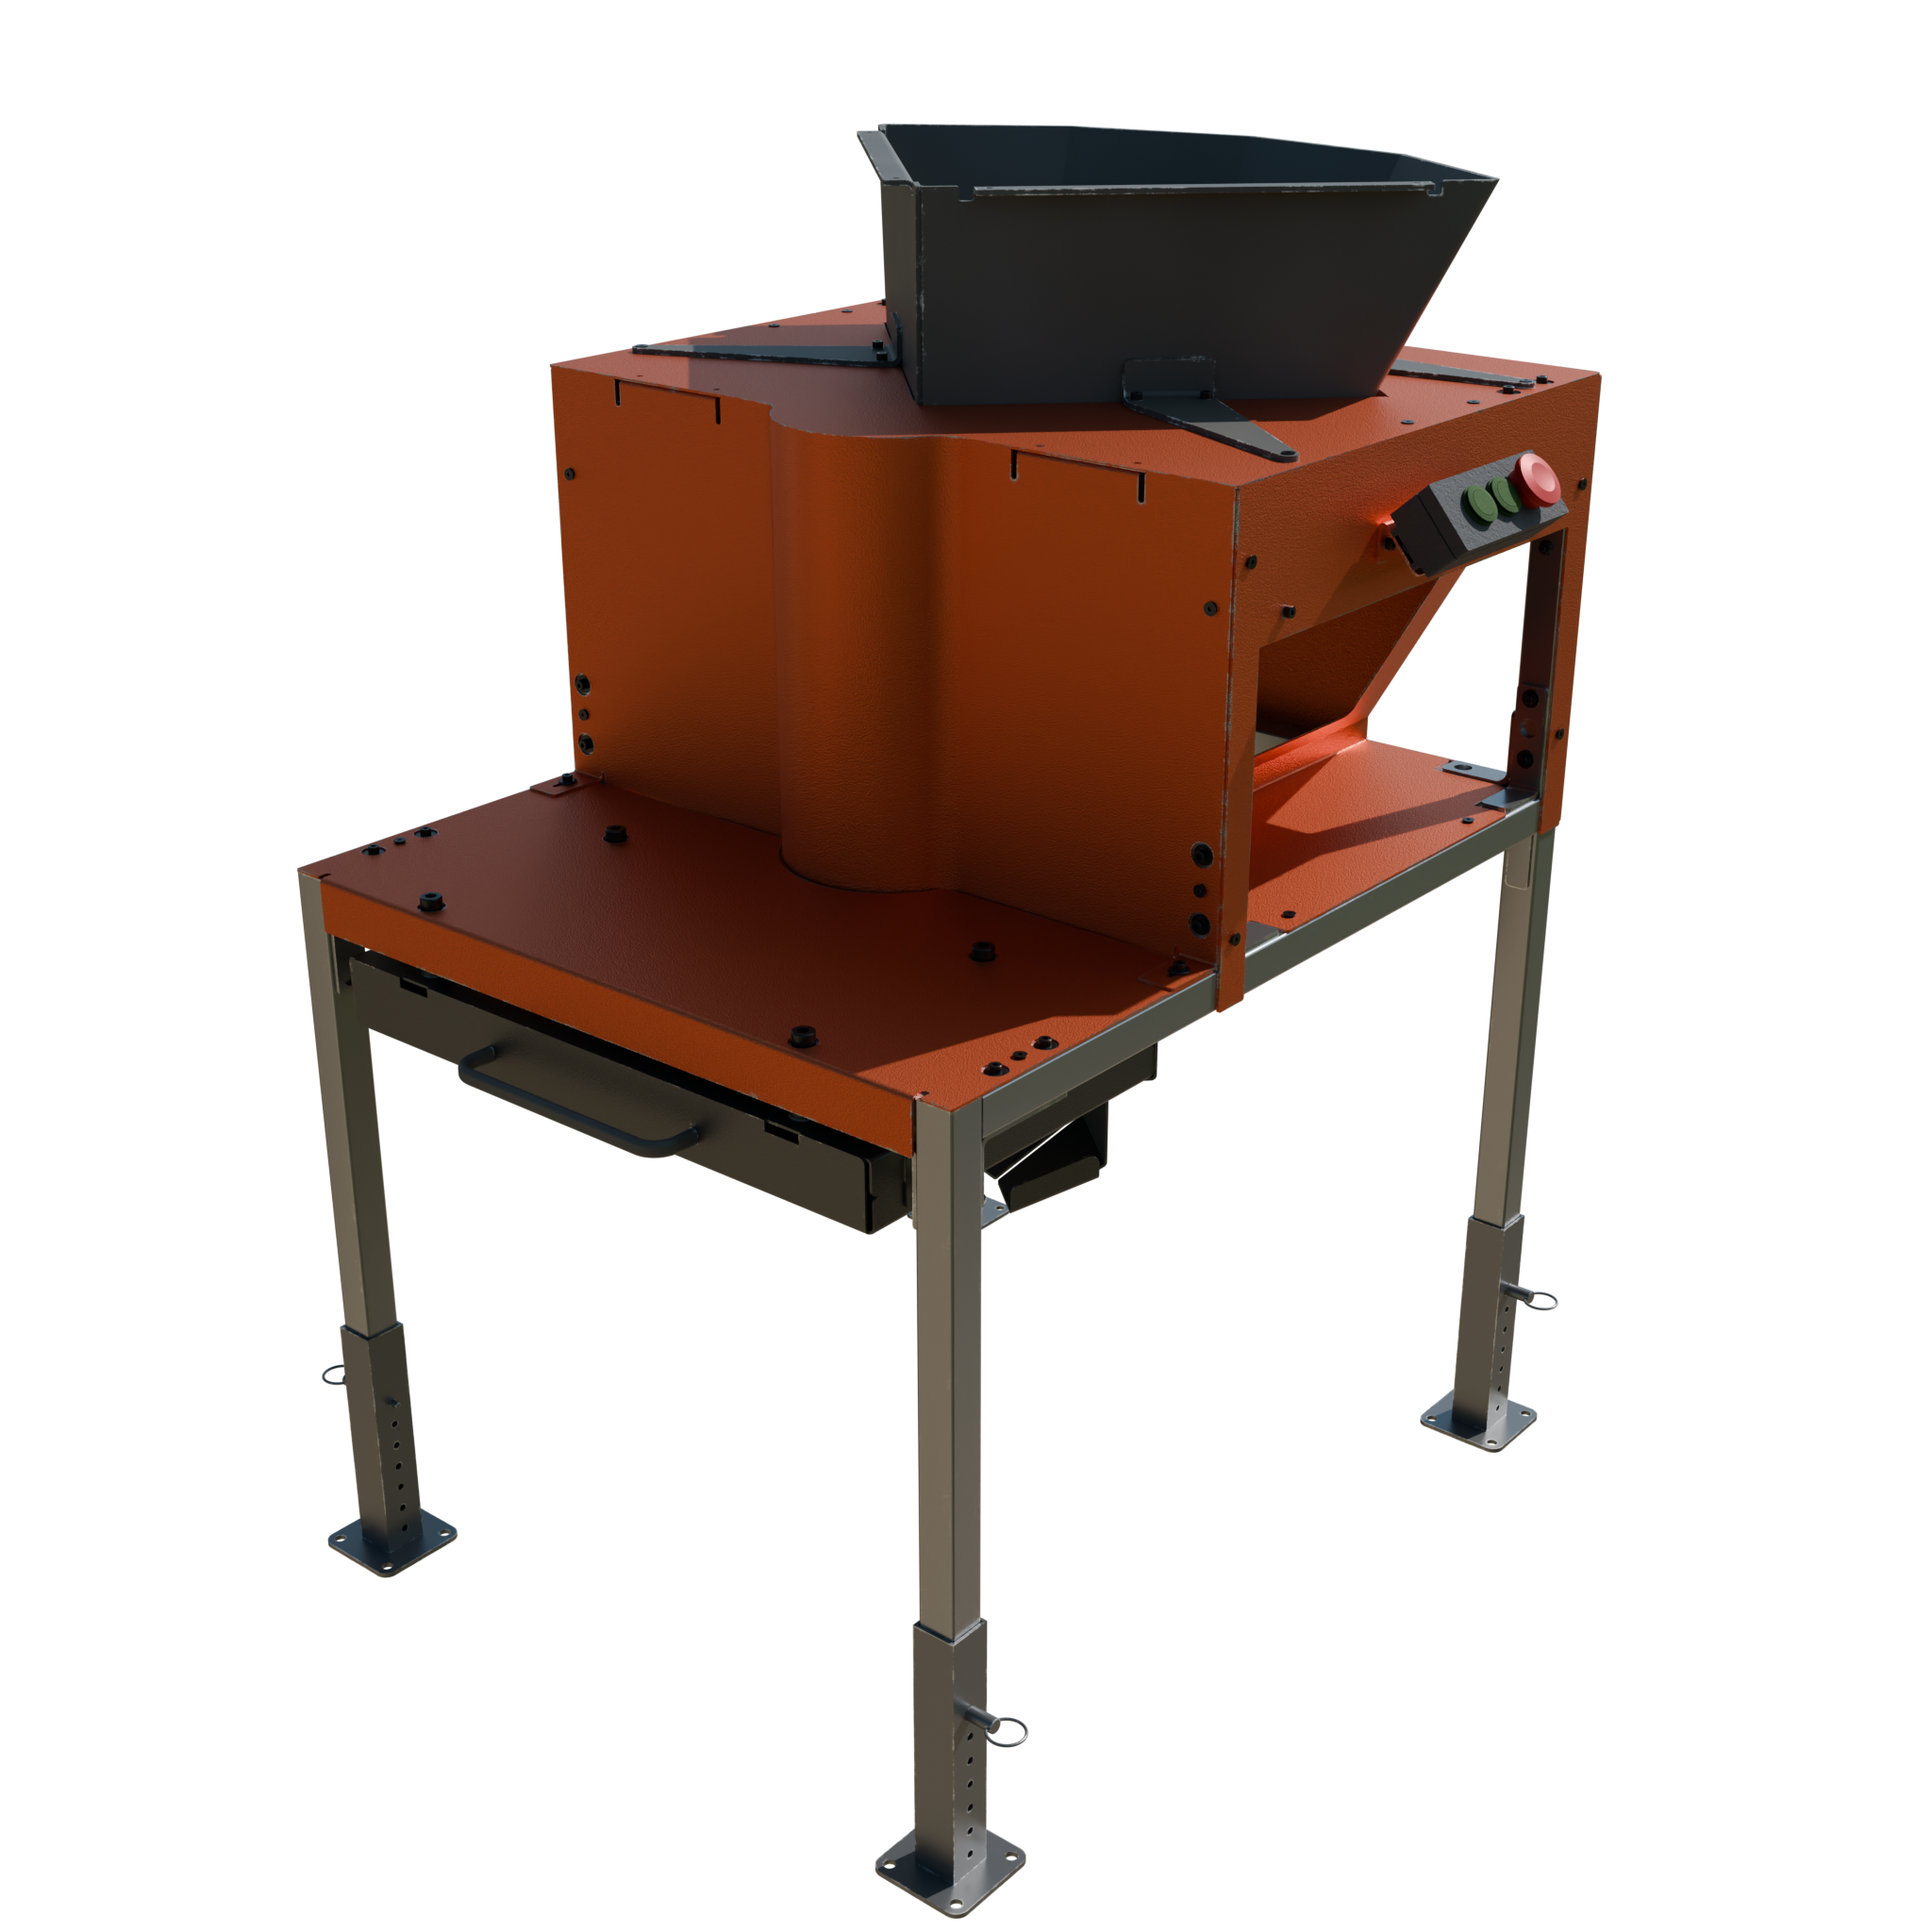
\includegraphics[width=0.5\textwidth]{../images/general_vue.png}
        \end{center}
        \vfill
        {\color{mainblue}\large Date: \today}
    %\end{minipage}
\end{titlepage}

\newpage



\newpage

\section*{Nomenclature des Pièces}

\begin{center}
\begin{tabularx}{0.95\textwidth}{>{\centering\arraybackslash}m{2.5cm} X >{\centering\arraybackslash}m{2cm}}
\textbf{Image} & \textbf{Description} & \textbf{Quantité} \\
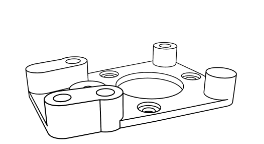
\includegraphics[width=2cm]{../images/part1.png} & Pièce A & 4 \\
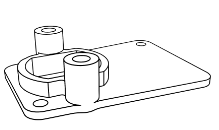
\includegraphics[width=2cm]{../images/part2.png} & Pièce B & 2 \\
& Pièce C & 1 \\
& Pièce D & 3 \\
& Pièce E & 5 \\
\end{tabularx}
\end{center}

\section*{Outils Nécessaires}
\begin{itemize}[label=\textbullet]
    \item Allen key
    \item Open-end wrench
\end{itemize}

\section*{Tool Usage Instructions}

\begin{enumerate}
    \item \textbf{Allen key:} Needed for hex screws.
    \begin{center}
        
\includegraphics[width=0.15\textwidth]{../images/tool2.png}
    \end{center}
    \item \textbf{Open-end wrench:} Needed for M5 nuts and Motor Nut.
    \begin{center}
        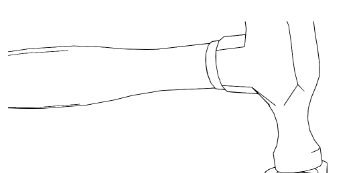
\includegraphics[width=0.15\textwidth]{../images/tool1.png}
    \end{center}
\end{enumerate}


\newpage


% En-tête de l'étape : numéro bien à gauche et en haut
\noindent
\begin{minipage}[t]{0.12\textwidth}
    \vspace*{-\topskip} % Remonte le contenu au maximum
    \raggedright
    \begin{tikzpicture}
        \node[anchor=north west] at (0,0) {\usefont{OT1}{phv}{b}{n}\huge 1}; % Numéro de l'étape
    \end{tikzpicture}
\end{minipage}%
\hfill

% !! images des pièces 
\begin{minipage}[t]{1\textwidth}
    \begin{tcolorbox}[colback=white, colframe=white!60, boxrule=0.7pt, left=2mm, right=2mm, top=1mm, bottom=1mm]
        \setlength{\extrarowheight}{0pt} % <-- Ajouté pour réduire l'espace vertical
        \begin{tabularx}{\textwidth}{@{}cc@{\hspace{1cm}}cc@{}}
            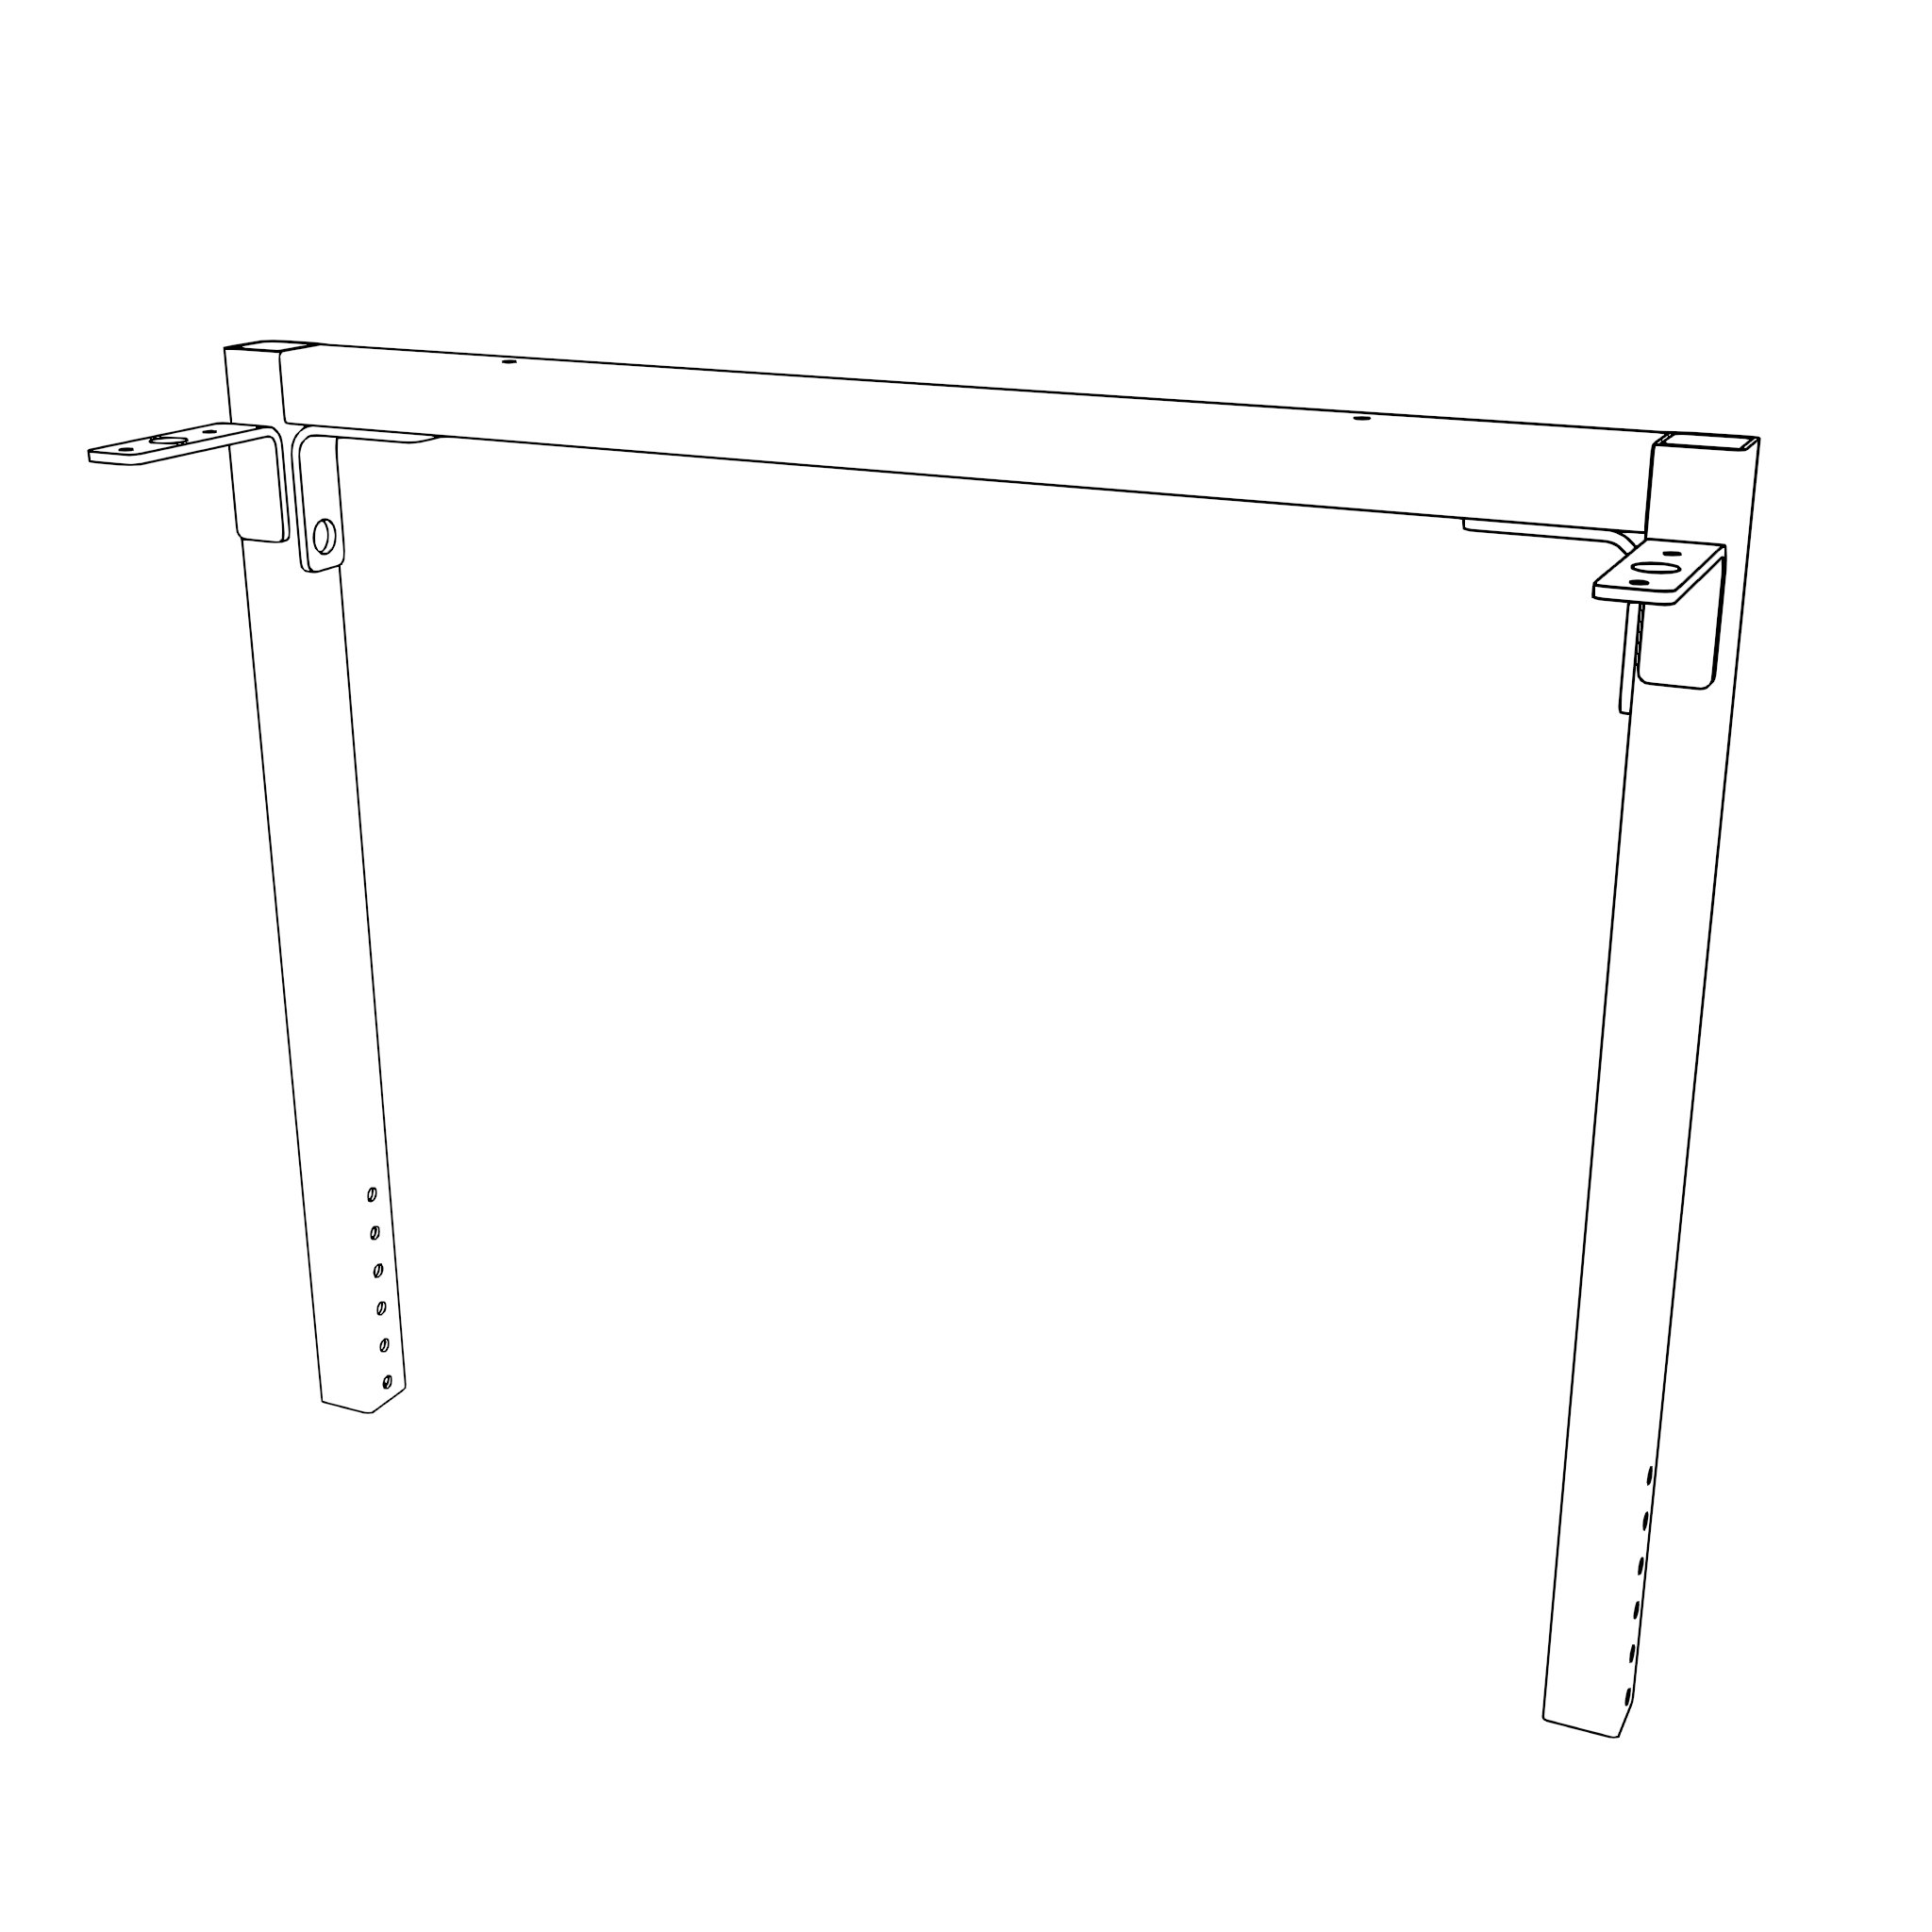
\includegraphics[width=2cm]{../images/_101_Pied Avant.png} & \textbf{Front legs} $\times$ 1
            & 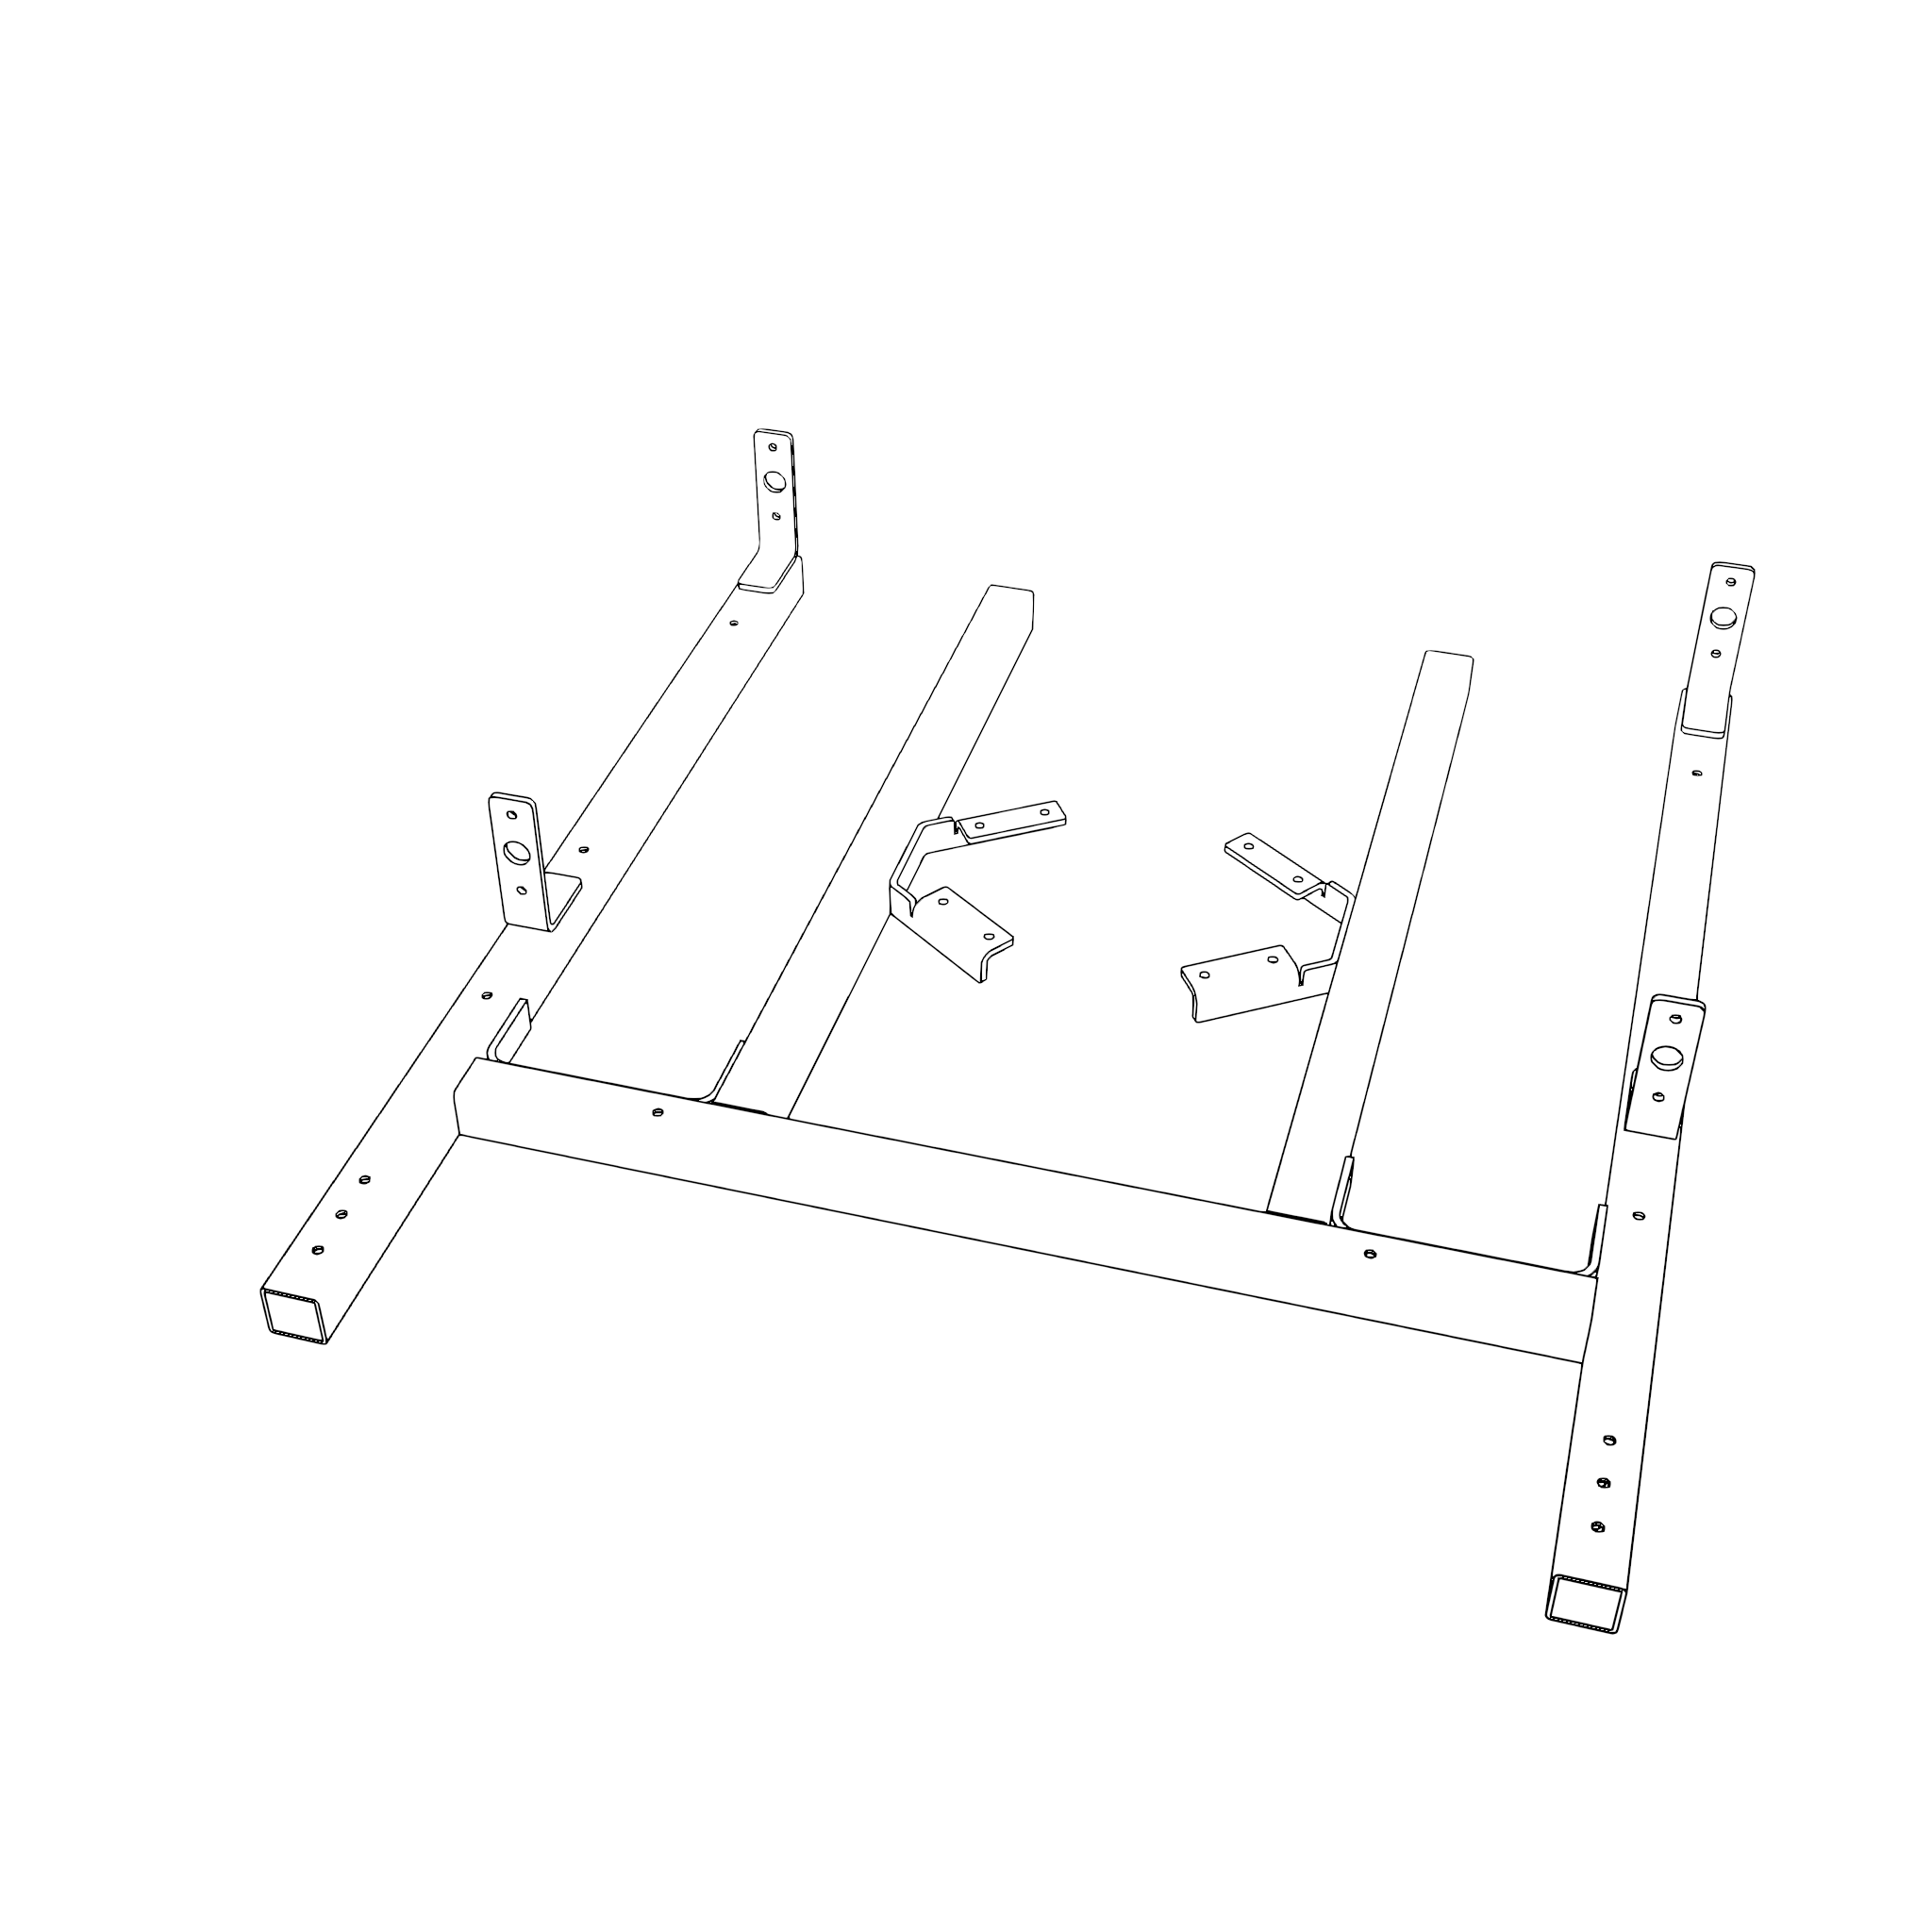
\includegraphics[width=2cm]{../images/_102_Plateau du Chassis.png} & \textbf{Chassis plate} $\times$ 1 \\
            %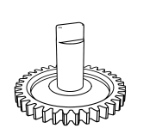
\includegraphics[width=1.5cm]{../images/part3.png} & \textbf{Pièce C} $\times$ 1
            %& & \\
        \end{tabularx}
        \setlength{\extrarowheight}{0.5em} % <-- Remet la valeur par défaut si besoin après
    \end{tcolorbox}


    % !! Images des outils centrées à droite
    \vspace{0.05em}
    \noindent
    \begin{flushright}
        %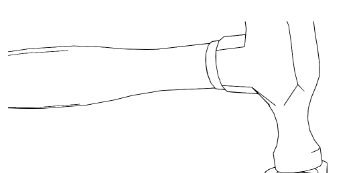
\includegraphics[height=1cm]{../images/tool1.png} \hspace{0.1cm}
        %
\includegraphics[height=1cm]{../images/tool2.png}
    \end{flushright}
\end{minipage}

\vspace{1em}

\begin{center}
    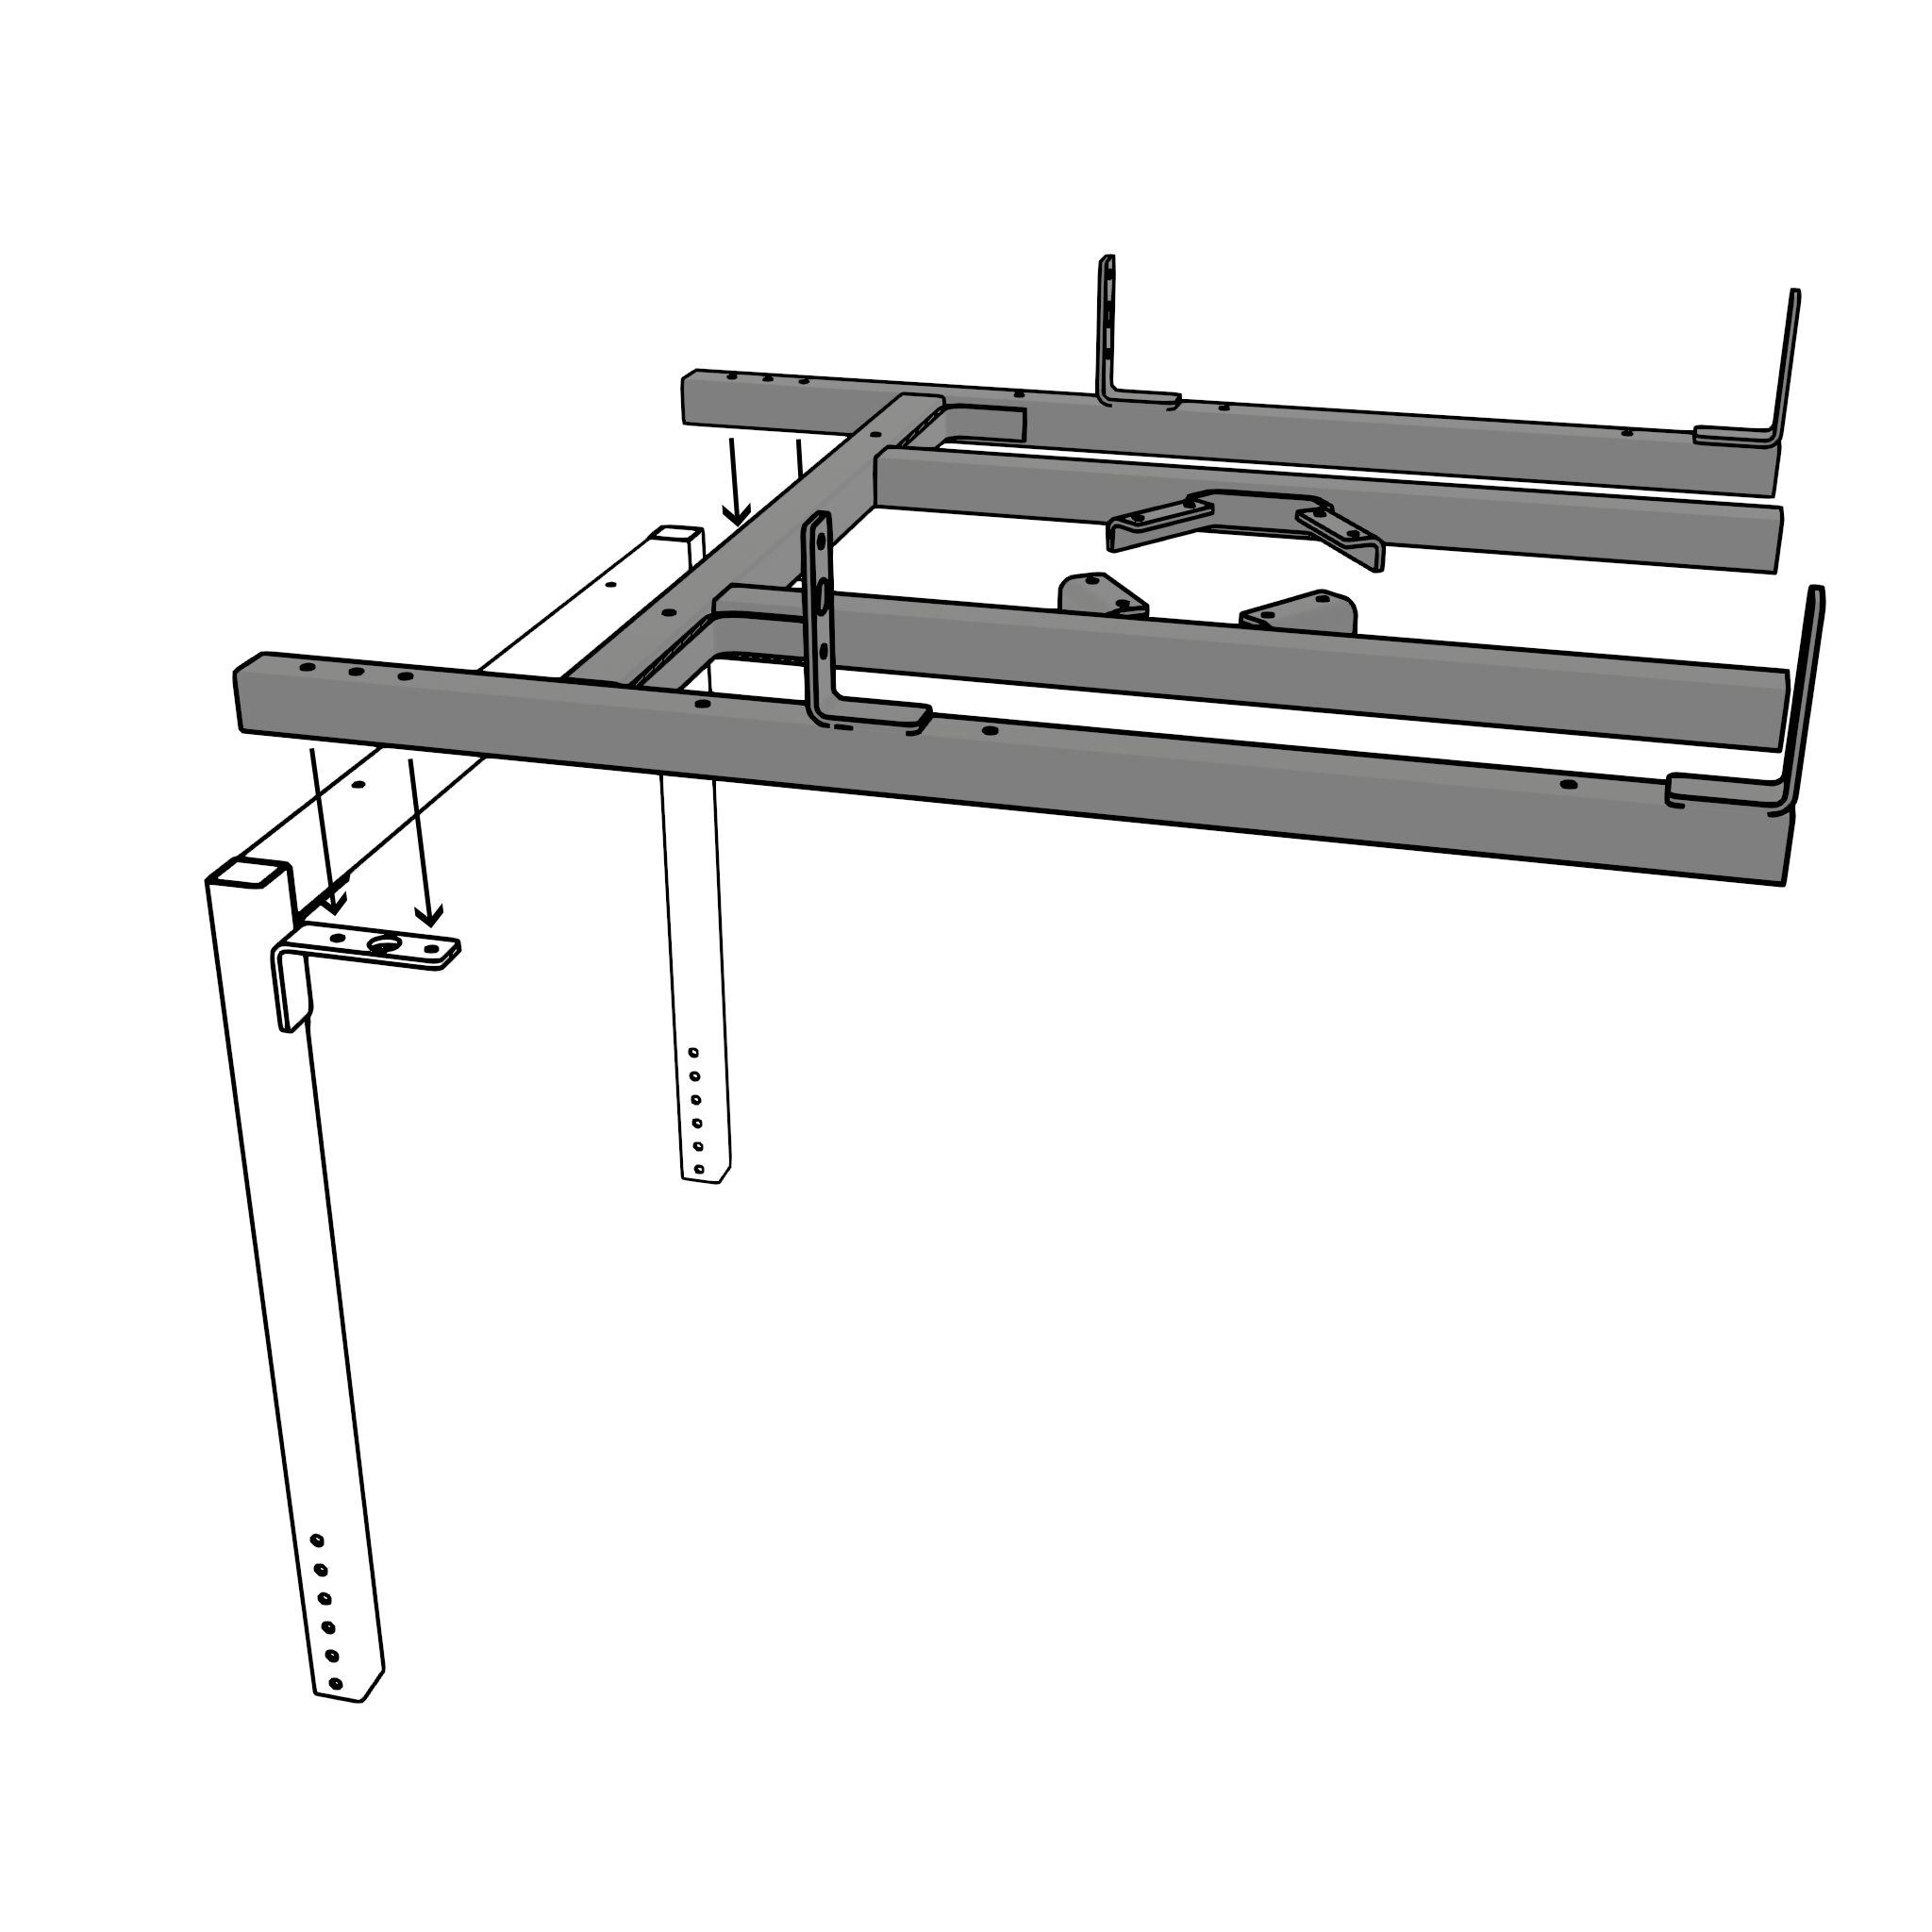
\includegraphics[height=12cm]{../images/_101_.png}
\end{center}

\vspace{0.7em}

%\begin{tcolorbox}[colback=gray!05, colframe=gray!60, boxrule=0.5pt, left=2mm, right=2mm, title=]
%    \begin{enumerate}
%        \item Rassemblez les pièces nécessaires (voir la nomenclature).
%        \item Allignez le pied avant avec le plateau du châssis.
%    \end{enumerate}
%\end{tcolorbox}


\newpage



% En-tête de l'étape : numéro bien à gauche et en haut
\noindent
\begin{minipage}[t]{0.12\textwidth}
    \vspace*{-\topskip} % Remonte le contenu au maximum
    \begin{tikzpicture}
        \node[anchor=north west] at (0,0) {\usefont{OT1}{phv}{b}{n}\huge 2}; % Numéro de l'étape
    \end{tikzpicture}
\end{minipage}%
\hfill

% !! images des pièces 
\begin{minipage}[t]{1\textwidth}
    \begin{tcolorbox}[colback=white, colframe=white!60, boxrule=0.7pt, left=2mm, right=2mm, top=1mm, bottom=1mm]
        \setlength{\extrarowheight}{0pt} % <-- Ajouté pour réduire l'espace vertical
        \begin{tabularx}{\textwidth}{@{}cc@{\hspace{1cm}}cc@{}}
            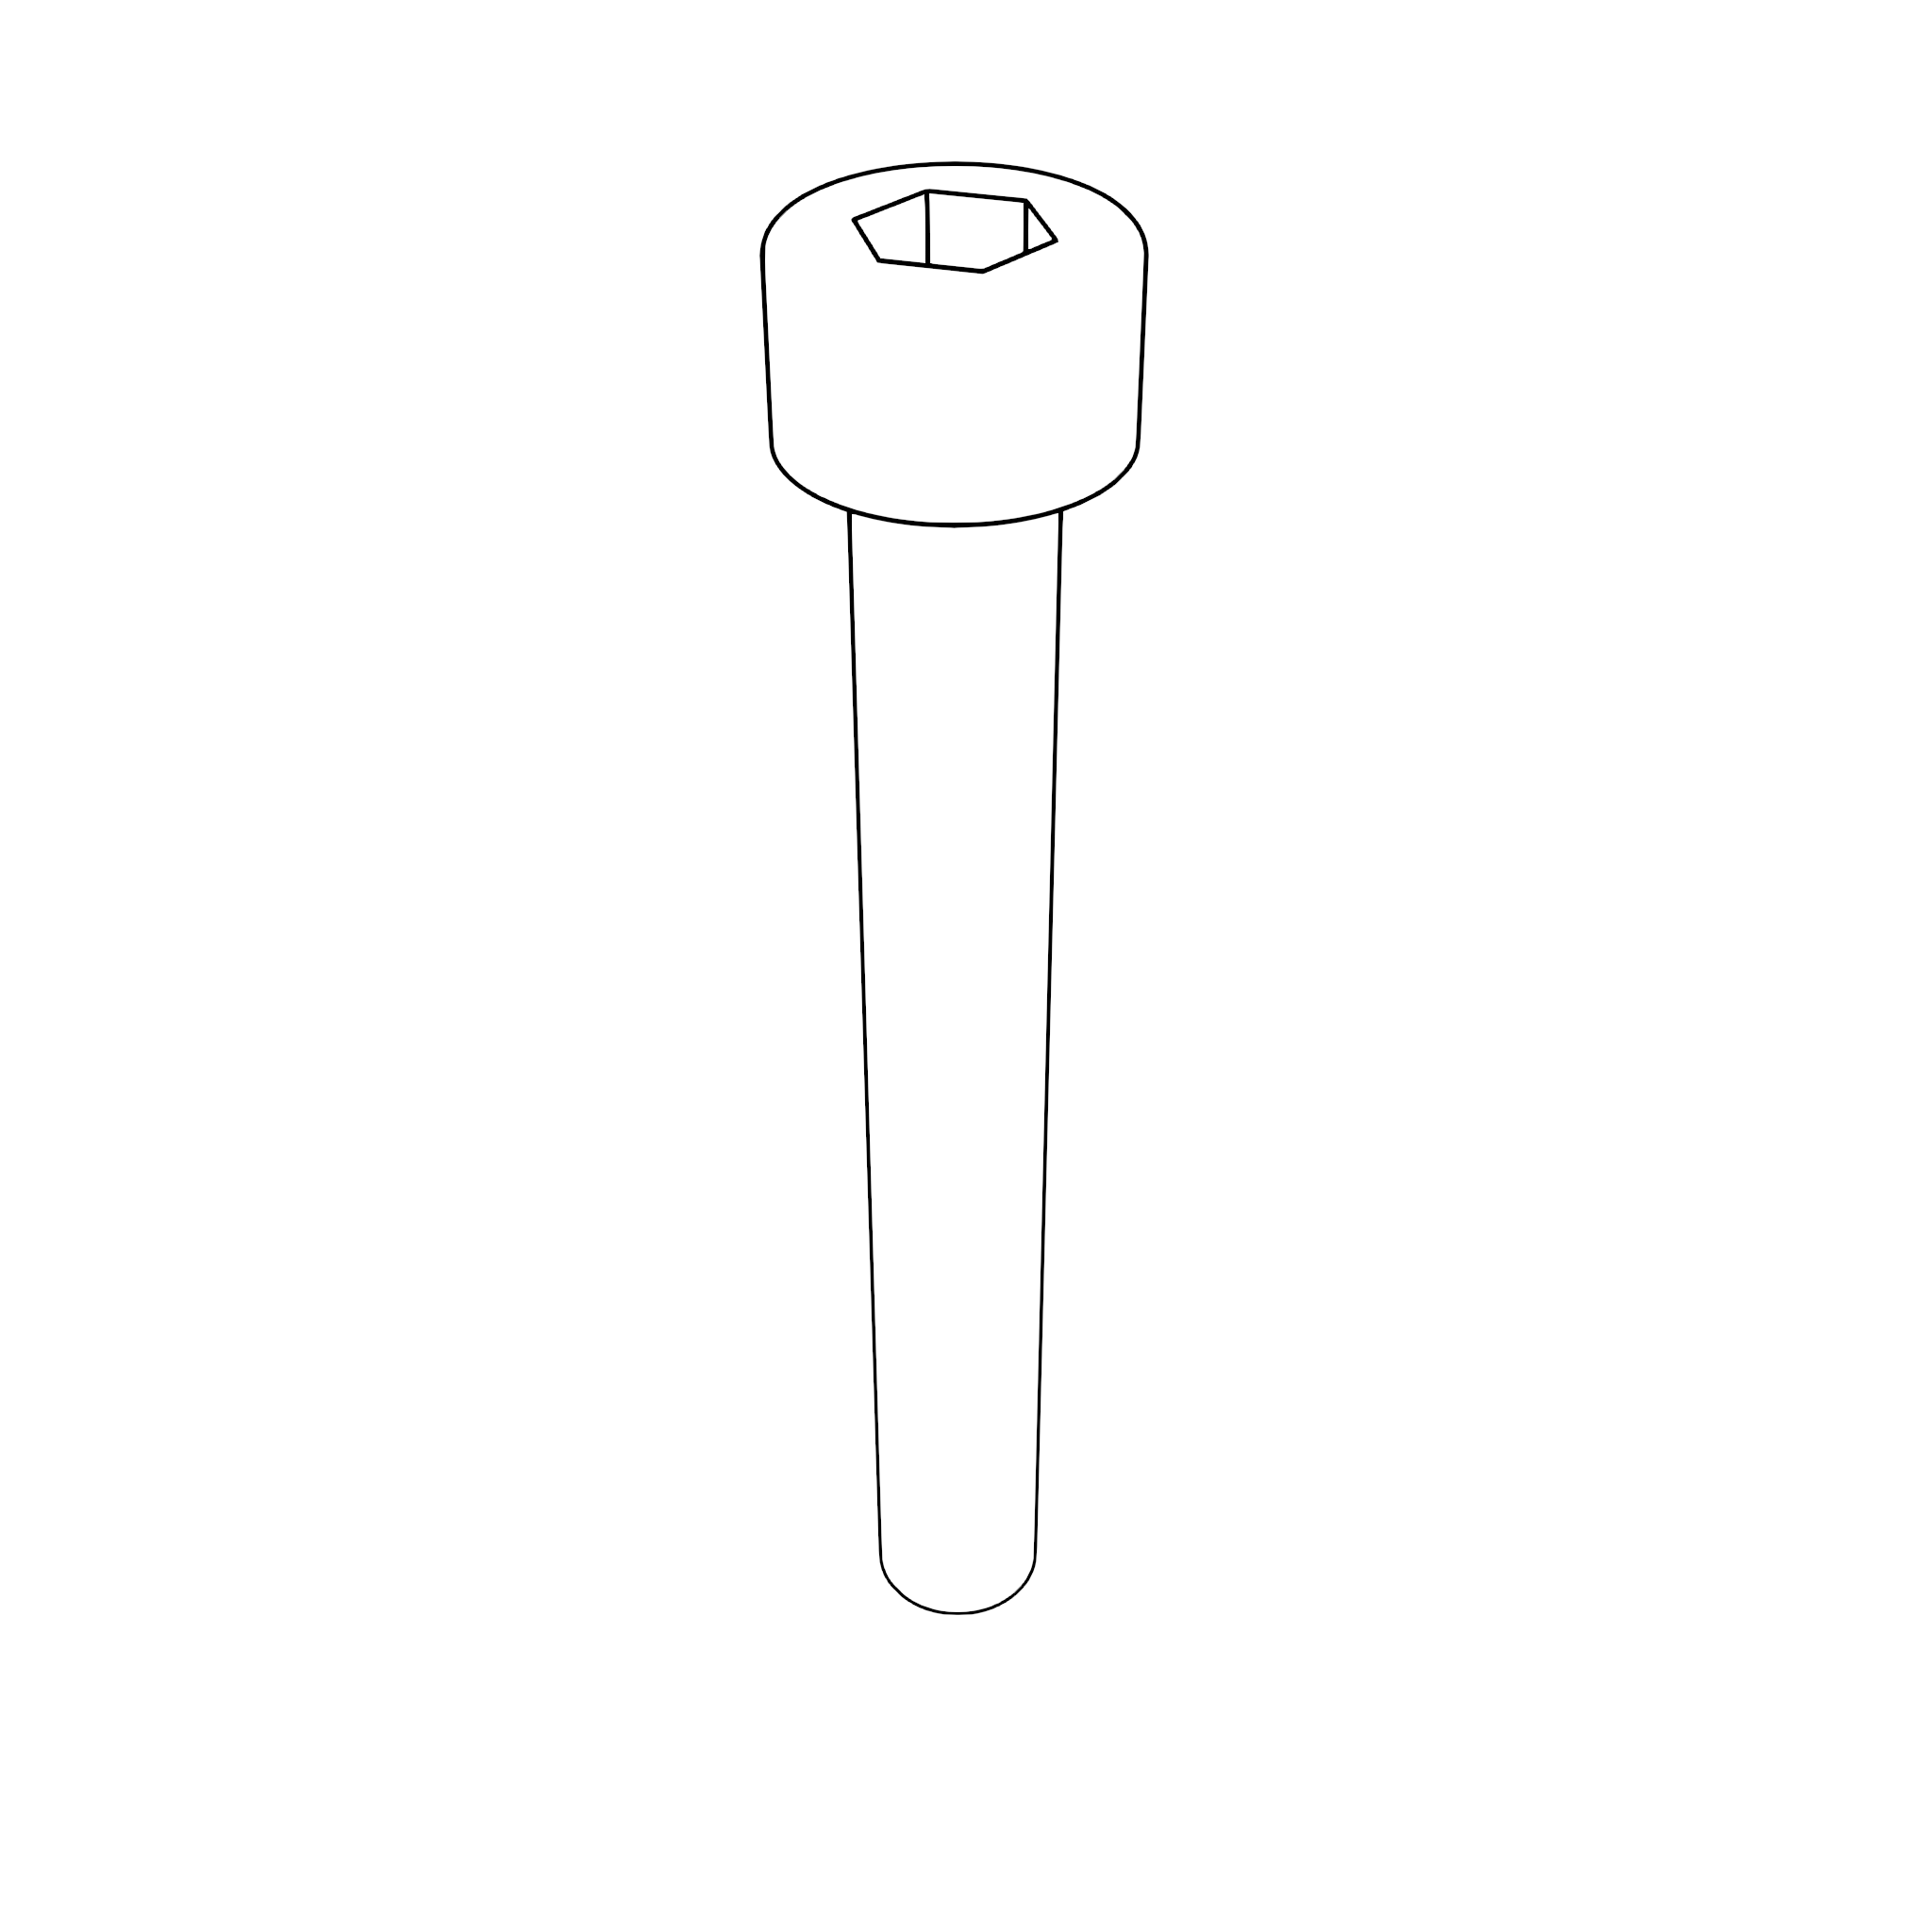
\includegraphics[width=1.5cm]{../images/_107_Vis.png} & \textbf{M5 Screw} $\times$ 2
            & 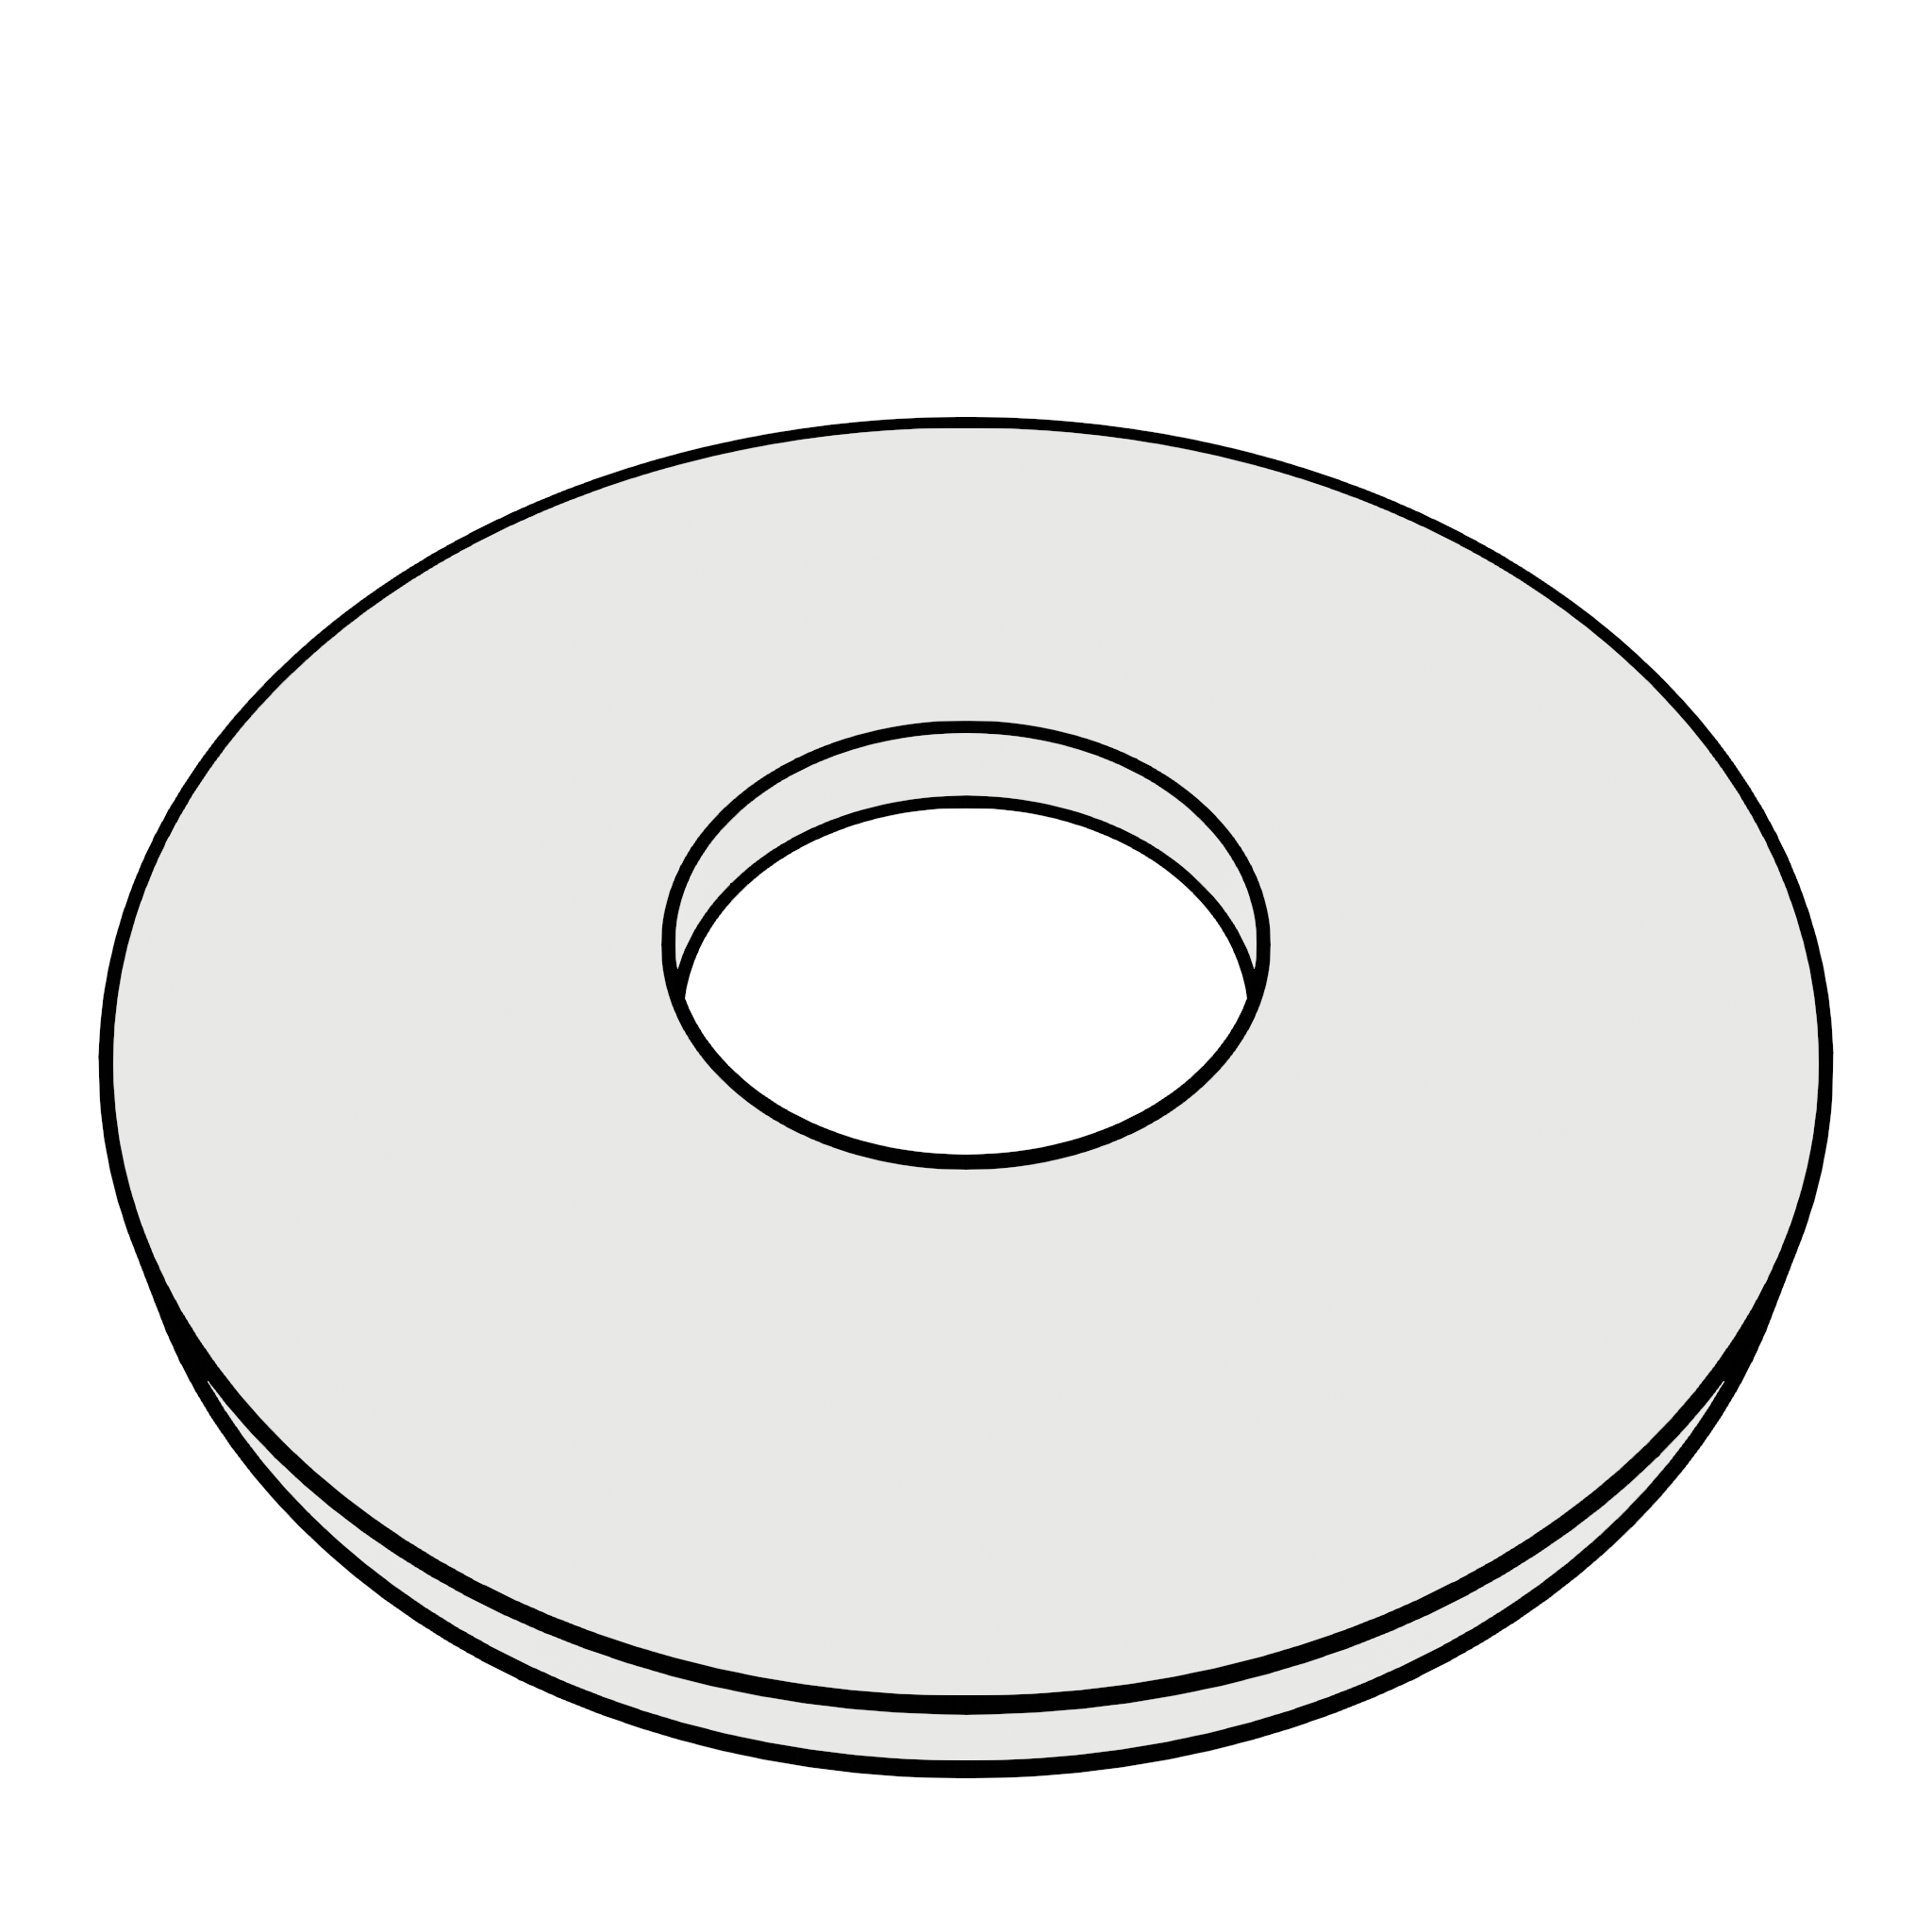
\includegraphics[width=1.5cm]{../images/_107_Rondele.png} & \textbf{Washer} $\times$ 2 \\
            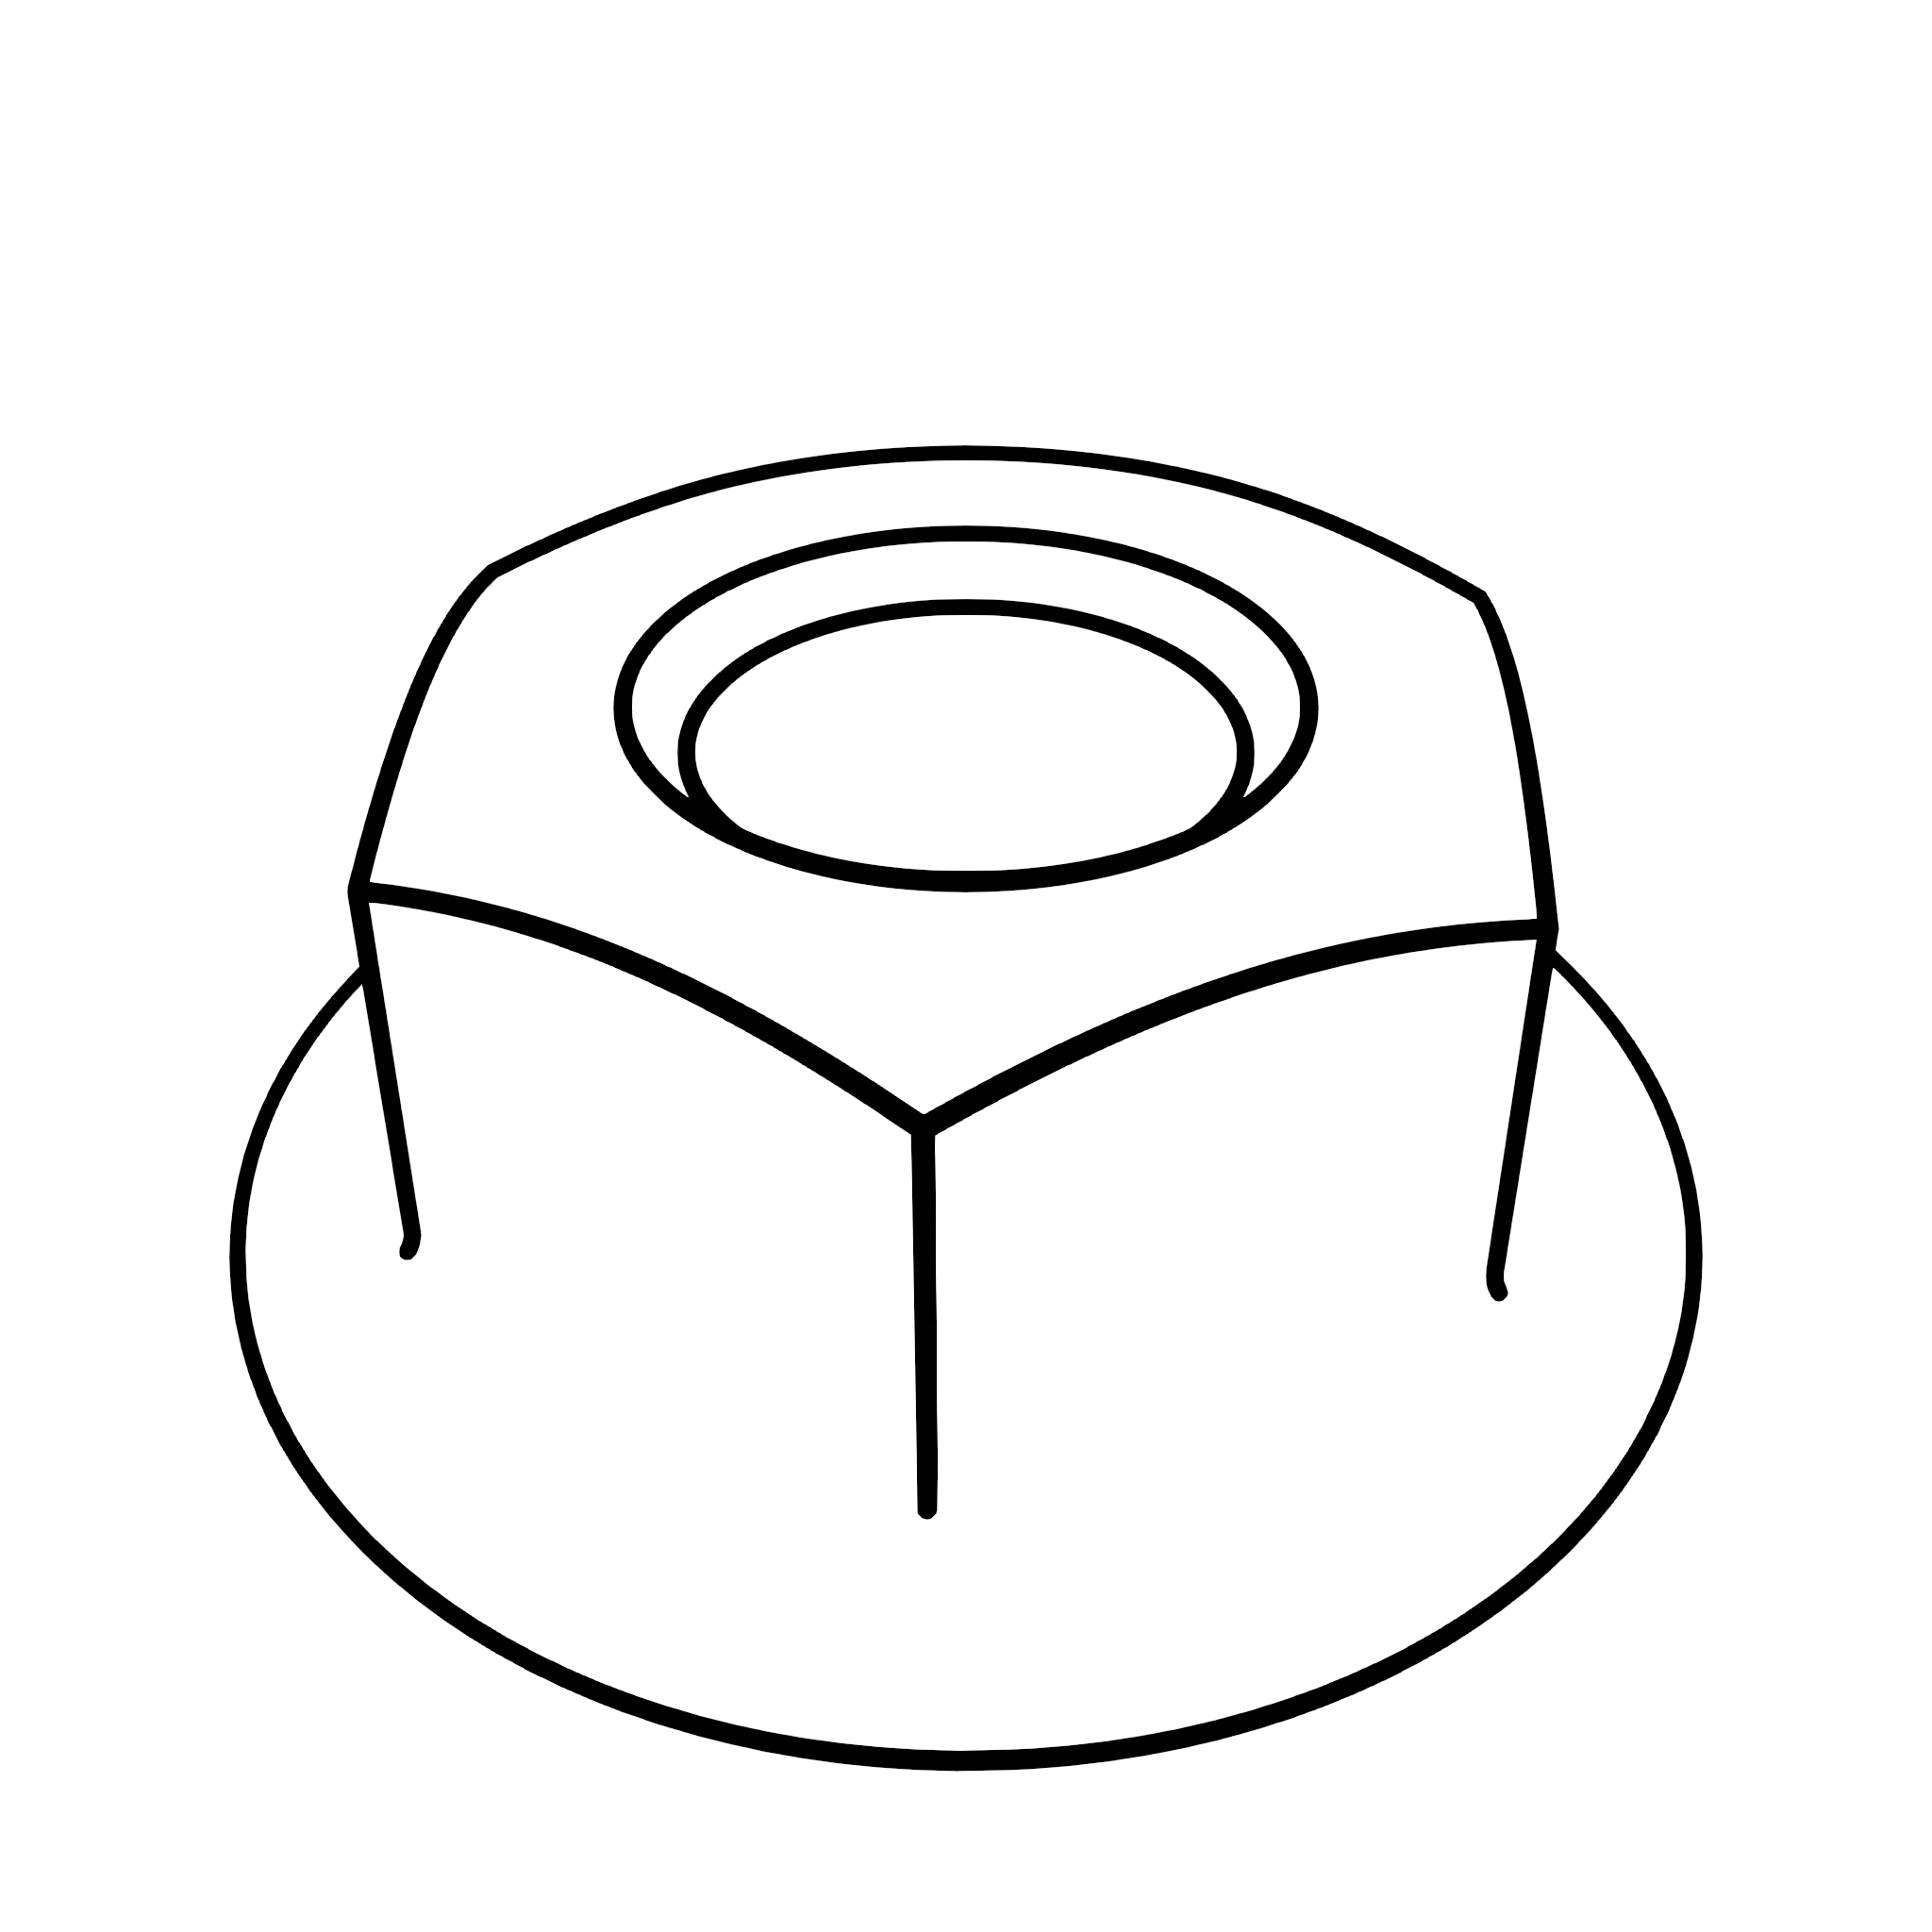
\includegraphics[width=1.5cm]{../images/_107_Nut.png} & \textbf{M5 Nut} $\times$ 2
            %& & \\
        \end{tabularx}
        \setlength{\extrarowheight}{0.5em} % <-- Remet la valeur par défaut si besoin après
    \end{tcolorbox}


    % !! Images des outils centrées à droite
    \vspace{0.05em}
    \noindent
    \begin{flushright}
        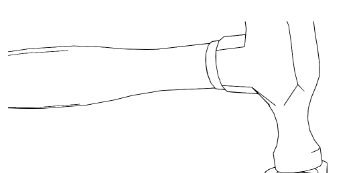
\includegraphics[height=1cm]{../images/tool1.png} \hspace{0.1cm}
        
\includegraphics[height=1cm]{../images/tool2.png}
    \end{flushright}
\end{minipage}

\vspace{1em}

\begin{center}
    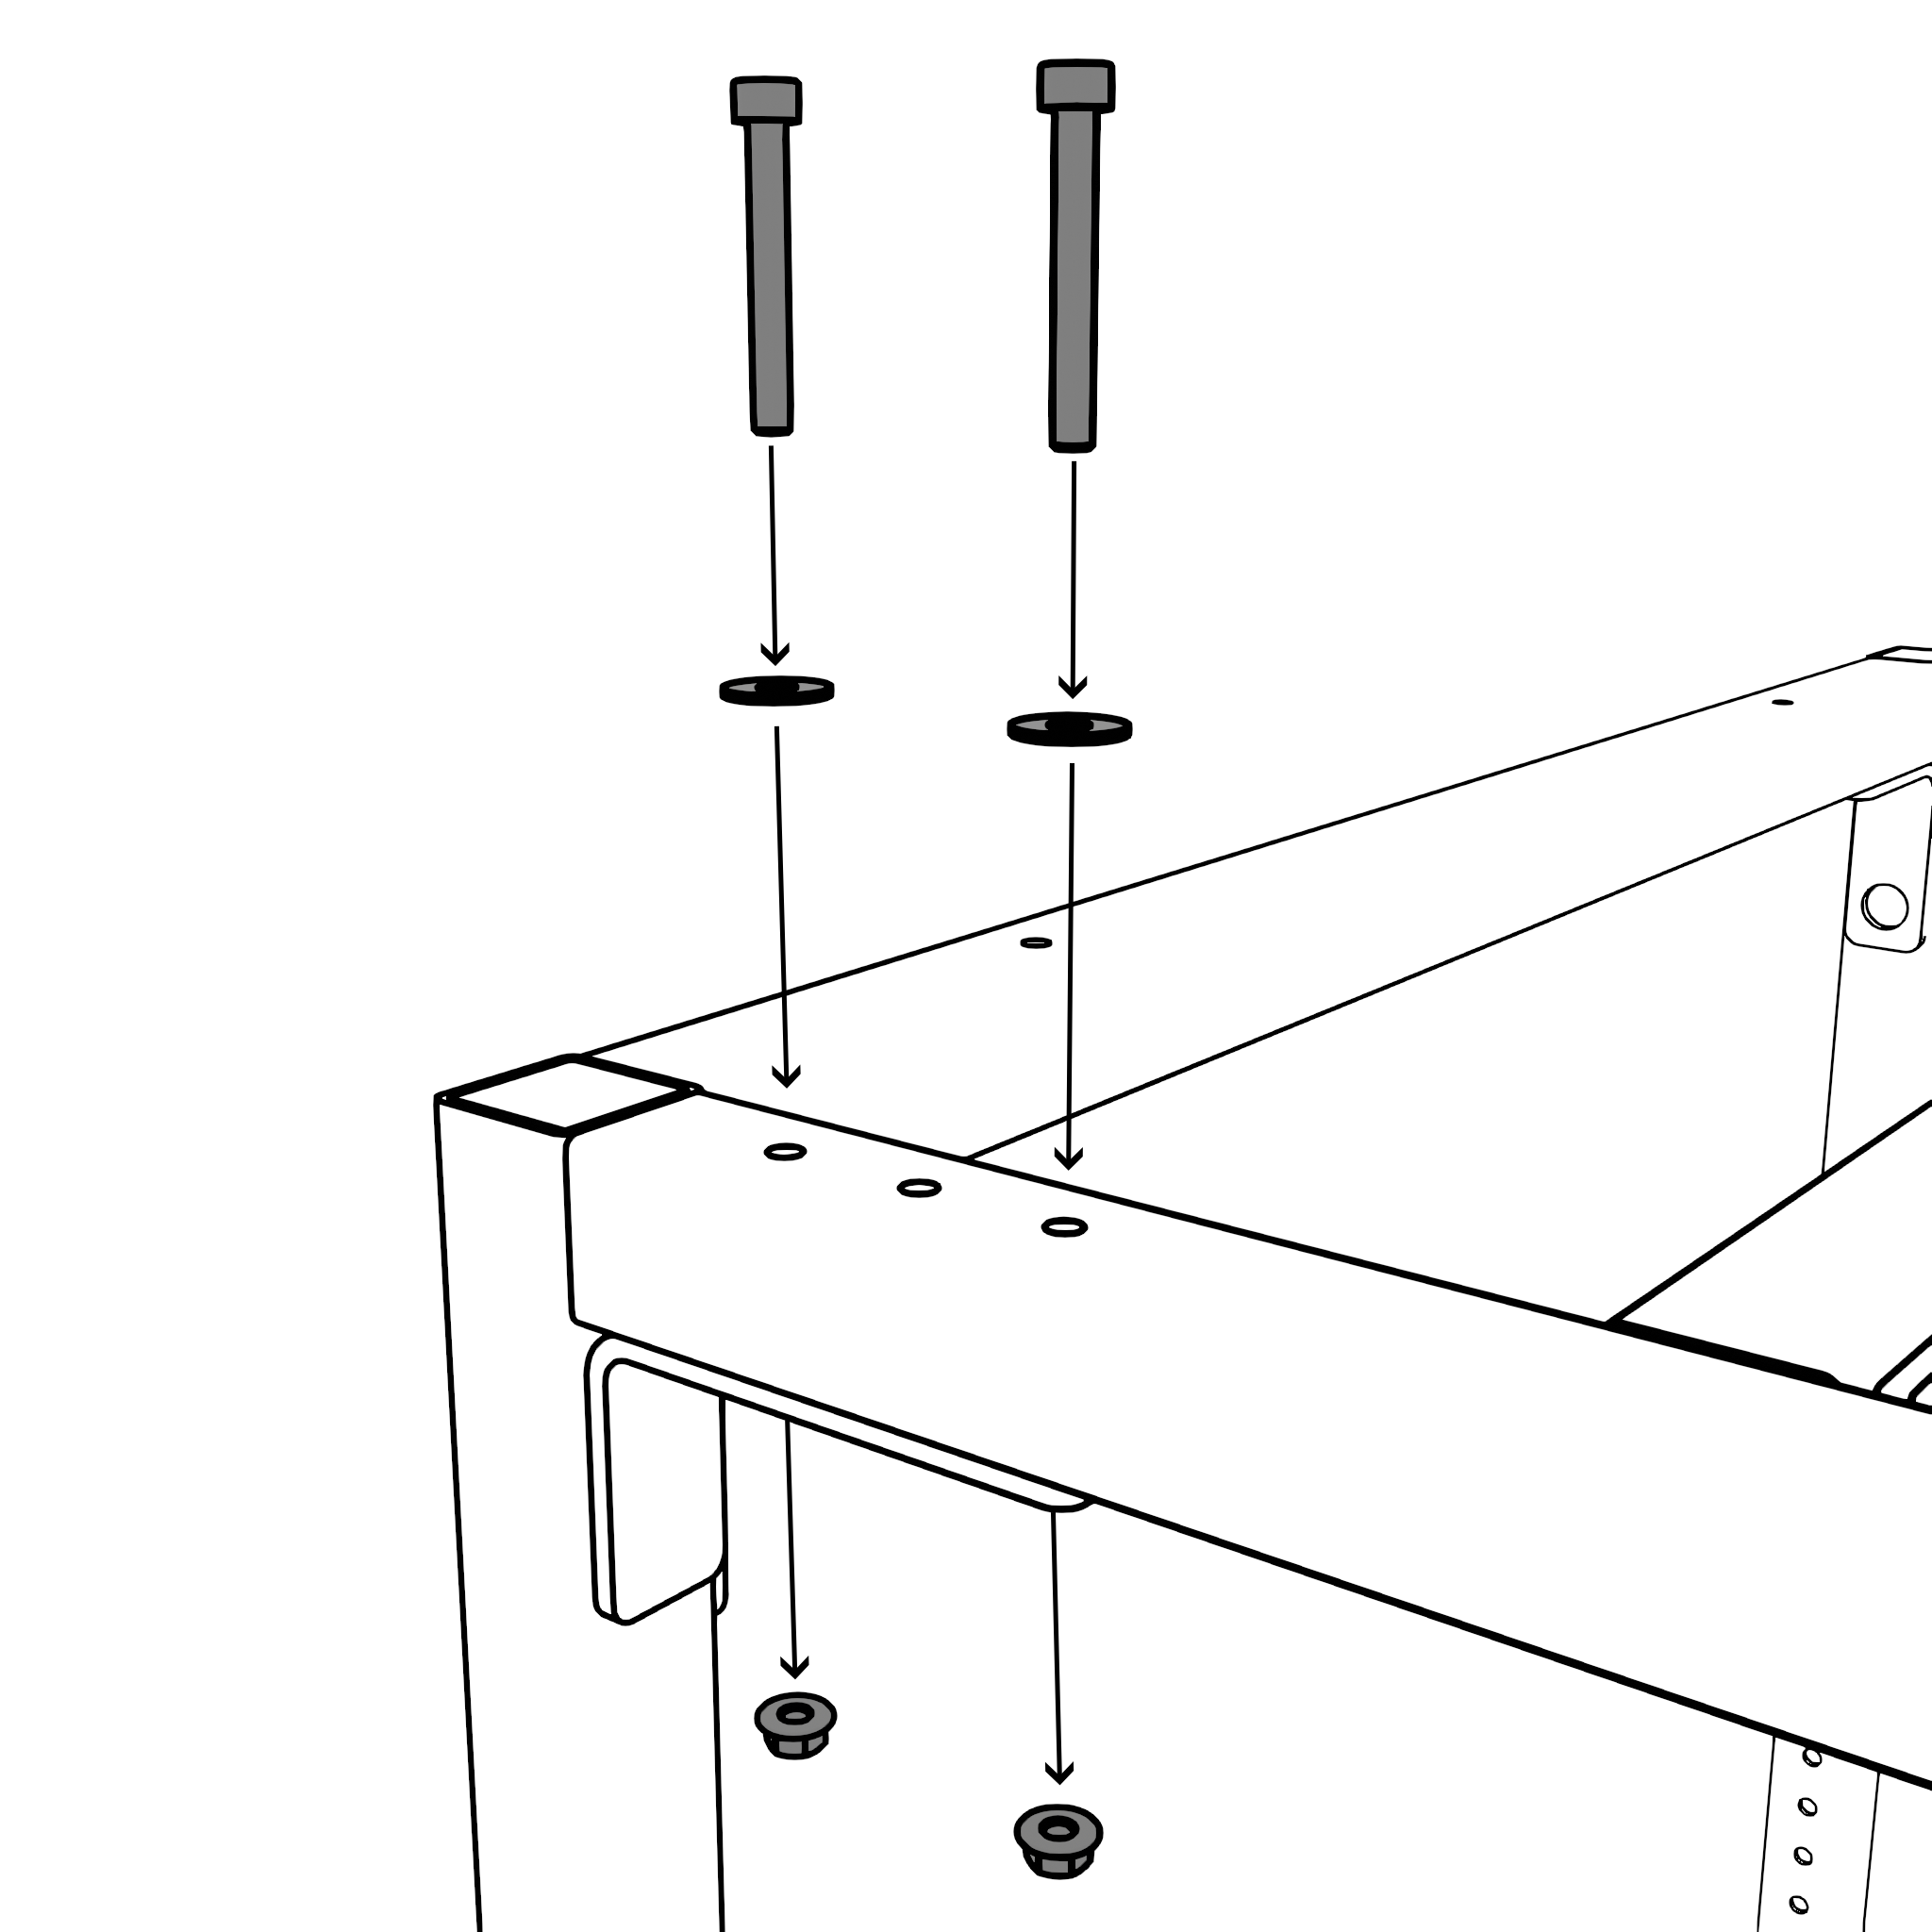
\includegraphics[height=10cm]{../images/_102_.png}
\end{center}

\vspace{0.7em}

%\begin{tcolorbox}[colback=gray!05, colframe=gray!60, boxrule=0.5pt, left=2mm, right=2mm, title=]
%    \begin{enumerate}
%        \item Rassemblez les pièces nécessaires (voir la nomenclature).
%        \item Vérifiez l'allignement entre le pied avant et le plateau du châssis.
%        \item Insérez les vis M5 à travers le pied avant et le plateau du châssis.
%        \item Serrzez les écrous M5 sur les vis.
%        \end{enumerate}
%\end{tcolorbox}


\newpage

\end{document}